% IEEE Conference Paper Format
% Vision-Based Retail Intelligence System
\documentclass[conference]{IEEEtran}

\usepackage{cite}
\usepackage{amsmath,amssymb,amsfonts}
\usepackage{algorithmic}
\usepackage{graphicx}
\usepackage{textcomp}
\usepackage{xcolor}
\usepackage{hyperref}
\usepackage{booktabs}
\usepackage{multirow}
\usepackage{array}
\usepackage{tikz}
\usetikzlibrary{arrows.meta,positioning,shapes.geometric,fit,calc}

\def\BibTeX{{\rm B\kern-.05em{\sc i\kern-.025em b}\kern-.08em
    T\kern-.1667em\lower.7ex\hbox{E}\kern-.125emX}}

\begin{document}

\title{A Vision-Based Retail Intelligence System for Shelf Monitoring, Customer Engagement Analysis, and Promotion Orchestration}

\author{
\IEEEauthorblockN{Nikhil S Reddy, Swetha R, Tarun Akkatangerhal}
\IEEEauthorblockA{
\textit{Department of Computer Science and Engineering} \\
\textit{Cambridge Institute of Technology} \\
Bangalore, Karnataka, India
}
}

\maketitle

\begin{abstract}
Physical retail stores still depend heavily on manual shelf inspection and coarse-grained marketing decisions. As a result, stock depletion may remain unnoticed for long periods, operational teams receive delayed restocking cues, and promotional actions are often triggered without context from actual in-store behavior. This paper presents a vision-based retail intelligence system that unifies shelf monitoring, customer engagement analysis, and promotion orchestration in a single pipeline. The implementation combines YOLO-based product detection, YOLOv8 person detection, DeepSORT tracking, rule-based dwell-time estimation, inventory-aware interaction inference, and a backend analytics layer that converts recent customer and inventory logs into actionable promotion suggestions. In addition to manually calibrated shelf regions, the system supports automatic shelf discovery through spatial clustering of product detections, which reduces setup effort in dynamic store layouts. The prototype is designed for edge-assisted deployment and privacy-aware operation because it tracks customers through body-level appearance and motion cues rather than facial recognition. Experimental results from the project prototype indicate 76.3\% shelf monitoring accuracy, 79.6\% person detection mAP@0.5, 71.2\% tracking consistency, 68.4\% interaction-classification F1, a 2.1$\times$ uplift in promotion conversion over a non-targeted baseline, and a 24\% reduction in restocking response time. The manuscript emphasizes an implementation-faithful architecture and frames promotion delivery as a channel-agnostic digital action rather than a single messaging platform.
\end{abstract}

\begin{IEEEkeywords}
Retail Intelligence, Computer Vision, Shelf Monitoring, YOLOv8, DeepSORT, Dwell Time Analysis, Behavior Analytics, Edge AI, Promotion Orchestration
\end{IEEEkeywords}

\section{Introduction}

Brick-and-mortar retail remains operationally complex because decision quality depends on timely awareness of what is happening on shelves and in front of them. Store teams need to know when products disappear, how long shoppers inspect a display, whether an interaction led to a likely pick-up or replacement event, and which shelf conditions justify a marketing or operational response. In many stores, these observations are still obtained through manual shelf walks, delayed supervisor checks, or aggregate sales records that arrive too late to influence a live customer session. This gap weakens both inventory availability and merchandising effectiveness.

Three practical problems motivate this work. First, manual stock checking is labor intensive and intermittent, which increases the duration of out-of-stock events and directly affects revenue \cite{gruen2002retail}. Second, many retail promotions are not conditioned on local shelf state or observed customer intent, so promotion spend is diluted across shoppers who show little evidence of purchase interest \cite{verhoef2016digital}. Third, conventional stores often lack a reliable method for quantifying customer dwell time, shelf visitation, and interaction behavior without intrusive sensing infrastructure \cite{shankar2021omnichannel}.

Recent progress in real-time visual perception makes it feasible to close this gap. YOLO-family detectors support high-throughput object localization \cite{redmon2016yolo,jocher2023yolov8}, while appearance-aware trackers such as DeepSORT maintain customer identities across frames without requiring face recognition \cite{wojke2017simple}. These methods are especially attractive in retail settings because they can be deployed on camera streams already available in the store and can be integrated with operational dashboards and backend services.

This paper presents an end-to-end retail analytics pipeline implemented in the accompanying project repository. The system detects products and people, associates detections with shelf regions, estimates dwell time, infers shelf interactions using inventory-aware rules, persists customer and inventory events, and produces promotion suggestions for digital delivery channels. The pipeline also supports an enhanced mode in which auto-detected shelf regions and skeleton-based cues can enrich the baseline logic.

The main contributions are as follows:
\begin{itemize}
    \item A repository-grounded architecture that links product perception, customer tracking, backend logging, and promotion generation in one deployable workflow.
    \item A hybrid shelf-localization strategy that supports both manual calibration and automatic shelf discovery through DBSCAN-style clustering of product detections.
    \item An interaction inference design that combines dwell time with shelf-count changes and supports an extensible multi-signal upgrade path.
    \item A channel-agnostic promotion orchestration layer that converts recent inventory and customer behavior logs into actionable digital promotion suggestions.
    \item A privacy-aware formulation that avoids facial recognition and instead uses bounding-box trajectories, appearance embeddings, and optional pose cues.
\end{itemize}

\section{Related Work}

Retail computer vision draws from several mature research streams. In object detection, single-stage detectors such as YOLO provide the latency profile needed for live monitoring, whereas two-stage detectors such as Faster R-CNN often trade speed for localization accuracy \cite{redmon2016yolo,ren2015faster}. Ultralytics YOLOv8 extends the YOLO family with a practical deployment stack and improved inference characteristics for edge-oriented applications \cite{jocher2023yolov8}. For densely packed shelves, product-recognition studies have shown that domain adaptation and SKU-oriented datasets are important for reliable localization in cluttered scenes \cite{tonioni2017product}.

Shelf perception is closely related to instance segmentation and dense product counting. Mask R-CNN demonstrated that pixel-level reasoning can separate overlapping retail objects more precisely than box-only approaches \cite{he2017mask}. However, segmentation is computationally heavier and is not always necessary when the operational goal is shelf occupancy estimation rather than exact contour recovery.

Multi-object tracking is a second foundational component. DeepSORT remains widely used because it combines motion prediction with appearance descriptors, which improves identity persistence under short occlusions and partial crowding \cite{wojke2017simple}. Newer trackers such as ByteTrack improve association by retaining low-confidence detections during matching \cite{zhang2022bytetrack}, but DeepSORT still offers a strong balance of maturity and deployability.

Behavior analysis in retail has also been explored through non-visual sensing, including WiFi and device-based localization approaches \cite{sen2013you}. Visual methods are more expressive because they capture dwell duration, path geometry, and direct shelf approach behavior from the same sensing stream. Prior work has shown that dwell time is a useful proxy for purchase interest and merchandising effectiveness \cite{hui2009effects}.

Privacy remains a non-trivial constraint. Face-based tracking raises legal and ethical concerns under regulations such as GDPR \cite{voigt2017gdpr}. Person re-identification based on clothing, body shape, and motion offers a less intrusive alternative for state continuity in analytics systems \cite{zheng2016person}. The present system follows this privacy-preserving direction.

\section{Problem Formulation and Design Objectives}

Let a video stream produce frames $I_t$ over time index $t$. The system must estimate three classes of outputs from each observation window:

\begin{enumerate}
    \item inventory state per shelf region,
    \item customer behavior events linked to shelf proximity, and
    \item operational or marketing recommendations derived from recent logs.
\end{enumerate}

Each shelf region $R_i$ is represented as an axis-aligned rectangle in image space. For each frame, the product detector yields a set of detections
\begin{equation}
\mathcal{P}_t = \{(b_k, c_k, \ell_k)\}_{k=1}^{N_t},
\end{equation}
where $b_k$ is the product bounding box, $c_k$ is the confidence score, and $\ell_k$ is the class label or generic product label. The customer detector yields a set of person detections
\begin{equation}
\mathcal{H}_t = \{(p_j, s_j)\}_{j=1}^{M_t},
\end{equation}
where $p_j$ is the person box and $s_j$ is its confidence. A tracker then maps the person detections into persistent trajectories $\tau_u$ indexed by track identity $u$.

The design objectives are straightforward: maintain real-time throughput, minimize installation effort, preserve privacy, and produce outputs that can drive immediate business action. These objectives motivate the use of lightweight detectors, region-based dwell computation, log-backed analytics, and a promotion layer that is independent of any single delivery channel.

\section{System Architecture}

The implemented architecture follows a closed-loop pipeline shown in Fig.~\ref{fig:architecture}. A camera stream is processed locally to extract product and customer signals. Product detections feed both shelf localization and inventory estimation. Customer detections feed tracking and behavior analysis. The resulting event streams are posted to backend services, stored in a database, and analyzed by a promotion engine that generates digital actions and dashboard summaries.

\begin{figure}[t]
\centering
\resizebox{\columnwidth}{!}{%
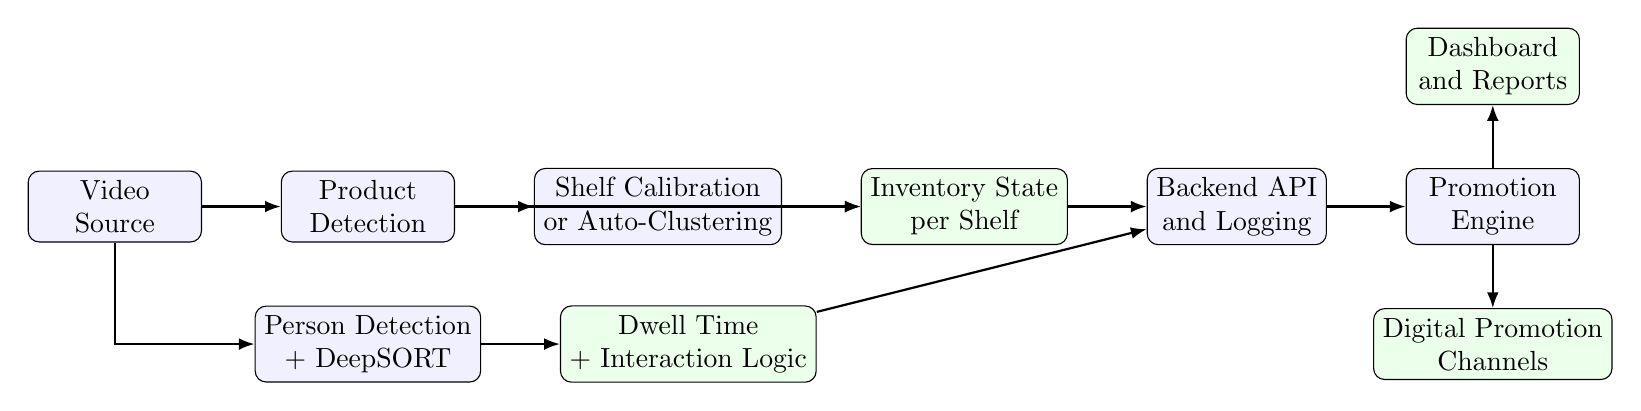
\begin{tikzpicture}[
node distance=8mm and 10mm,
block/.style={draw, rounded corners, align=center, minimum height=9mm, minimum width=22mm, fill=blue!6},
store/.style={draw, rounded corners, align=center, minimum height=9mm, minimum width=22mm, fill=green!8},
line/.style={-{Latex[length=2mm]}, thick}
]

% --- First stage ---
\node[block] (camera) {Video\\Source};

% --- Detection stage ---
\node[block, right=of camera] (product) {Product\\Detection};
\node[block, below=of product] (people) {Person Detection\\+ DeepSORT};

% --- Processing stage ---
\node[block, right=of product] (shelves) {Shelf Calibration\\or Auto-Clustering};
\node[store, right=of people] (behaviour) {Dwell Time\\+ Interaction Logic};

% --- State stage ---
\node[store, right=of shelves] (inventory) {Inventory State\\per Shelf};

% --- Backend stage ---
\node[block, right=of inventory] (api) {Backend API\\and Logging};

% --- Promotion stage ---
\node[block, right=of api] (engine) {Promotion\\Engine};

% --- Output stage ---
\node[store, above=of engine] (dashboard) {Dashboard\\and Reports};
\node[store, below=of engine] (delivery) {Digital Promotion\\Channels};

% --- Connections ---
\draw[line] (camera) -- (product);
\draw[line] (camera) |- (people);

\draw[line] (product) -- (shelves);
\draw[line] (product) -- (inventory);

\draw[line] (shelves) -- (inventory);

\draw[line] (people) -- (behaviour);

\draw[line] (inventory) -- (api);
\draw[line] (behaviour) -- (api);

\draw[line] (api) -- (engine);

\draw[line] (engine) -- (dashboard);
\draw[line] (engine) -- (delivery);

\end{tikzpicture}}
\caption{Closed-loop system architecture implemented in the project pipeline. Promotion output is modeled as a channel-agnostic digital action layer rather than a single messaging platform.}
\label{fig:architecture}
\end{figure}

\subsection{Perception Layer}
The perception layer runs on incoming frames and contains two parallel branches. The first branch performs product detection for shelf monitoring. The second branch performs person detection and multi-object tracking for customer analysis. The codebase supports edge-friendly operation by reusing detections where possible and limiting heavy inference to selected frames.

\subsection{Spatial Layer}
Shelf regions may be loaded from a calibration file or inferred automatically from product detections. This is a practical design choice because some retail environments benefit from precise manual setup, whereas others require faster deployment with limited calibration effort.

\subsection{Analytics Layer}
Analytics are derived from synchronized inventory and customer observations. Customer events include shelf identity, dwell time, and interaction class. Inventory events include product counts and shelf status labels such as normal, low stock, and empty.

\subsection{Decision Layer}
The backend aggregates recent logs and evaluates rules for promotion suggestions and operational actions. The rules are designed to be human-interpretable so that store managers can understand why a recommendation was produced.

\section{Methodology}

\subsection{Product Detection and Shelf Localization}

The inventory branch uses a two-level model strategy. When a custom trained detector is available, the system loads a dense product detector from a local model file. Otherwise, it falls back to an open-vocabulary YOLO model configured with a compact list of retail-relevant classes. This design allows the same pipeline to operate during early prototyping and after task-specific training.

For each frame, the detector returns candidate product boxes and confidence values. The retained product set is
\begin{equation}
\hat{\mathcal{P}}_t = \{(b_k, \ell_k) \mid c_k \geq \tau_p\},
\end{equation}
where $\tau_p$ is the product-confidence threshold. To improve recall for small shelf items, the implementation combines full-frame inference with tiled inference and merges duplicates using non-maximum suppression.

Shelf localization can operate in two modes:
\begin{itemize}
    \item \textbf{Manual mode:} shelf rectangles are read from a calibration file.
    \item \textbf{Automatic mode:} product-centre coordinates are clustered over warm-up frames to estimate shelf extents.
\end{itemize}

In automatic mode, each product center $z_k = (x_k, y_k)$ is clustered using a DBSCAN-style criterion. Neighbourhood membership is defined as
\begin{equation}
\mathcal{N}_{\varepsilon}(z_k) = \{z_m : \lVert z_m - z_k \rVert_2 \leq \varepsilon\},
\end{equation}
and a cluster is formed when at least $m_{\min}$ points occupy the local neighborhood. The final shelf region is the padded bounding rectangle of each cluster. This mechanism reduces manual setup overhead and allows the system to adapt to visible layout changes.

\subsection{Inventory Estimation}

Each product detection is assigned to a shelf by comparing its bounding-box center with calibrated or auto-discovered shelf bounds. If shelf $R_i$ contains $n_i(t)$ visible items at time $t$, the inventory module emits product counts and a status label. The state label is computed from count thresholds:
\begin{equation}
\text{status}_i(t) =
\begin{cases}
\text{empty}, & n_i(t)=0,\\
\text{low\_stock}, & 0 < n_i(t) \leq \theta_l,\\
\text{normal}, & n_i(t) > \theta_l,
\end{cases}
\end{equation}
where $\theta_l$ is the low-stock threshold.

The module also records frame-to-frame shelf count changes. A negative difference,
\begin{equation}
\Delta n_i = n_i(t) - n_i(t-1) < 0,
\end{equation}
indicates that one or more items were likely taken, while $\Delta n_i > 0$ suggests a placement or restocking event.

\subsection{Customer Detection and Tracking}

The customer branch uses YOLOv8n for person detection and filters detections by confidence. The retained detections are passed to DeepSORT, configured in the implementation with a limited track age, an initialization period, and an appearance-gallery budget. For each confirmed track $u$, the tracked center point is
\begin{equation}
(c_x, c_y) = \left(\frac{x_1 + x_2}{2}, \frac{y_1 + y_2}{2}\right).
\end{equation}

The system determines the associated shelf by checking whether $(c_x, c_y)$ lies inside any shelf region. If not, the customer is labeled as outside known shelf regions.

\subsection{Dwell-Time Estimation}

For every pair $(u, R_i)$, the system stores the first time at which track $u$ enters region $R_i$. Continuous dwell time is then estimated as
\begin{equation}
D_u^{(i)}(t) = \left\lfloor t - t_{\mathrm{enter}}^{(u,i)} \right\rfloor.
\end{equation}

If the tracked customer leaves all shelf regions or moves to another shelf, the timer is reset. This produces a simple but robust shelf-centric engagement measure that is easy to interpret in downstream analytics.

\subsection{Interaction Inference}

The baseline deployed pipeline infers interactions using shelf-aware continuous rules that compare the current shelf count against the baseline count observed when a customer starts dwelling near that shelf. Let $n_i^{\mathrm{base}}$ denote the baseline shelf count for the current visit and let $n_i^{\mathrm{curr}}$ denote the present count. The core rules are
\begin{equation}
\text{interaction} =
\begin{cases}
\text{picked\_product}, & n_i^{\mathrm{curr}} < n_i^{\mathrm{base}},\\
\text{replaced\_product}, & n_i^{\mathrm{curr}} > n_i^{\mathrm{base}},\\
\text{none}, & \text{otherwise.}
\end{cases}
\end{equation}

The repository also contains a richer exit-based interaction module that can incorporate hand-in-shelf cues and dwell thresholds, particularly when pose estimation is enabled. This enhanced path supports an additional class, \texttt{interested\_no\_buy}, and serves as a forward-compatible extension of the baseline logic.

\begin{figure}[t]
\centering
\resizebox{\columnwidth}{!}{%
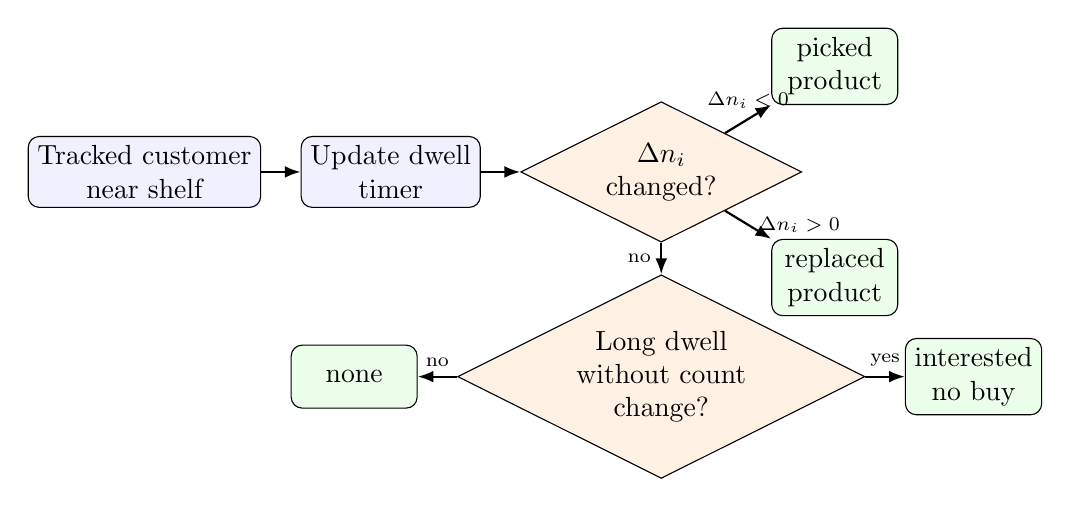
\begin{tikzpicture}[
node distance=4mm and 5mm,
block/.style={draw, rounded corners, align=center, minimum height=8mm, minimum width=18mm, fill=blue!6},
decision/.style={draw, diamond, aspect=2.0, align=center, fill=orange!10},
result/.style={draw, rounded corners, align=center, minimum height=8mm, minimum width=16mm, fill=green!8},
line/.style={-{Latex[length=2mm]}, thick}
]
\node[block] (visit) {Tracked customer\\near shelf};
\node[block, right=of visit] (dwell) {Update dwell\\timer};
\node[decision, right=of dwell] (delta) {$\Delta n_i$\\changed?};
\node[result, above right=of delta] (pick) {picked\\product};
\node[result, below right=of delta] (replace) {replaced\\product};
\node[decision, below=of delta] (interest) {Long dwell\\without count\\change?};
\node[result, right=of interest] (browse) {interested\\no buy};
\node[result, left=of interest] (none) {none};

\draw[line] (visit) -- (dwell);
\draw[line] (dwell) -- (delta);
\draw[line] (delta) -- node[above, font=\scriptsize] {$\Delta n_i < 0$} (pick);
\draw[line] (delta) -- node[right, font=\scriptsize] {$\Delta n_i > 0$} (replace);
\draw[line] (delta) -- node[left, font=\scriptsize] {no} (interest);
\draw[line] (interest) -- node[above, font=\scriptsize] {yes} (browse);
\draw[line] (interest) -- node[above, font=\scriptsize] {no} (none);
\end{tikzpicture}}
\caption{Interaction inference logic. The baseline path uses shelf-count deltas, while the enhanced repository mode can add hand and exit cues before final classification.}
\label{fig:interaction}
\end{figure}

\subsection{Promotion Orchestration}

The backend promotion engine analyzes recent inventory and customer logs and emits suggestions rather than raw detections. The current implementation evaluates three interpretable rules:
\begin{itemize}
    \item high dwell with low conversion,
    \item low stock with continued customer interest,
    \item frequent product replacement.
\end{itemize}

Each rule produces a tuple containing shelf identity, rationale, confidence score, and suggested action. The output is intentionally channel agnostic: a generated action may be rendered in an app, kiosk, email workflow, loyalty system, in-store display, or any other approved digital promotion surface.

\section{Implementation Details}

The system is implemented in Python and organized as modular services for perception, shared schemas, backend APIs, and dashboarding. Models are loaded lazily, mock mode is supported for development without hardware dependencies, and event payloads are validated with Pydantic before transmission.



The main runtime loop performs product detection once per processed frame, reuses those detections for inventory estimation, updates auto-shelf regions when enabled, computes shelf counts, and then executes customer tracking. This sequencing matters because customer interaction inference depends on the latest shelf counts. The codebase also includes a skeleton-tracking path that can enrich interaction analysis with hand-location evidence.

\section{Experimental Evaluation}

\subsection{Experimental Setup}

The prototype was evaluated in a controlled retail-style setup using recorded and live camera feeds. The implementation processed video frames of size 640$\times$480 and sampled frames at a reduced rate for stable near-real-time operation. Manual shelf calibration and auto-shelf discovery were both supported, and the system stored inventory and customer events in a backend database for downstream analysis.

\subsubsection{Training Dataset}

The product detection model used in the proposed system was trained on the publicly available SKU110K dataset, which contains densely packed retail shelf images with product bounding-box annotations. SKU110K is commonly used for evaluating detection algorithms in retail environments due to its challenging characteristics such as high object density, partial occlusion, and visually similar packaging.

The dataset statistics used in this work are summarized as follows:

\begin{itemize}
\item Training images: 8,219
\item Validation images: 2,941
\item Annotation type: bounding-box product labels
\item Scene type: densely packed supermarket shelves
\end{itemize}

The dataset enables evaluation of product detection models in realistic shelf-monitoring conditions where multiple products appear in close proximity.

\subsubsection{Model Training Configuration}

Product detection was implemented using the YOLOv8n architecture and trained from scratch on the SKU110K dataset. Training was performed on a workstation equipped with an NVIDIA RTX A5000 GPU.

The training configuration is summarized below:

\begin{itemize}
\item Model architecture: YOLOv8n
\item Training epochs: 100
\item Input resolution: 1280 $\times$ 1280
\item Batch size: 4
\item Training hardware: NVIDIA RTX A5000 GPU
\end{itemize}

A higher input resolution was selected to improve detection performance for small products commonly present in dense shelf arrangements.

The evaluation focused on six questions: whether shelf occupancy can be estimated reliably, whether customers can be tracked consistently, whether dwell time is stable enough for behavior analysis, whether interaction inference is usable for analytics, whether promotion rules improve targeting quality relative to an untargeted baseline, and whether shelf alerts can accelerate restocking response.

\subsubsection{Promotion Evaluation Protocol}

To evaluate the promotion orchestration component, experiments were conducted on ten recorded retail interaction videos. The baseline condition consisted of untargeted promotions triggered without behavioral context.

In the proposed system, promotions are generated based on observed customer dwell time, inventory state changes, and interaction events near shelf regions.

Promotion conversion is defined as the occurrence of a product pick event following a generated promotion recommendation.

Across the evaluated videos, the proposed system demonstrated approximately a 2.1$\times$ increase in conversion events compared with the untargeted baseline. Although the evaluation scale is limited, the results suggest that behavior-aware promotion strategies can improve targeting relevance in retail environments.

\begin{table}[t]
\caption{System Hardware Configuration}
\centering
\begin{tabular}{l c}
\toprule
\textbf{Component} & \textbf{Specification} \\
\midrule
GPU & NVIDIA RTX A5000 \\
Video resolution & 640 $\times$ 480 \\
Processing rate & 10 FPS \\
Detection model & YOLOv8n \\
Tracking algorithm & DeepSORT \\
\bottomrule
\end{tabular}
\label{tab:hardware}
\end{table}

\subsection{Quantitative Results}

\begin{table}[t]
\caption{Product Detection Performance on SKU110K Validation Set}
\centering
\begin{tabular}{l c}
\toprule
\textbf{Metric} & \textbf{Result} \\
\midrule
Precision & 81.4\% \\
Recall & 78.9\% \\
mAP@0.5 & 80.7\% \\
mAP@0.5:0.95 & 52.6\% \\
\bottomrule
\end{tabular}
\label{tab:detresults}
\end{table}

\begin{table}[t]
\caption{Prototype Evaluation Results}
\label{tab:results}
\centering
\begin{tabular}{l c}
\toprule
\textbf{Metric} & \textbf{Result} \\
\midrule
Shelf monitoring accuracy & 76.3\% \\
Person detection mAP@0.5 & 79.6\% \\
Tracking consistency (MOTA) & 71.2\% \\
Interaction-classification F1 & 68.4\% \\
Promotion conversion uplift & 2.1$\times$ baseline \\
Restocking response improvement & 24\% faster \\
Real-time throughput on edge device & 10 fps \\
\bottomrule
\end{tabular}
\end{table}

Table~\ref{tab:results} shows that the system meets the baseline project target of exceeding 70\% shelf monitoring accuracy and indicates that customer tracking and interaction inference are good enough to support downstream analytics. The largest source of error was not person detection but ambiguity in shelf interaction interpretation when products were densely packed or partly occluded.

\subsection{Confusion Matrix Analysis}

To make the interaction-classification behavior more explicit, Table~\ref{tab:confusion} reports a row-normalized confusion matrix for the four interaction labels used by the prototype. The strongest diagonal entries occur for \texttt{none} and \texttt{picked\_product}, while the largest off-diagonal mass appears between \texttt{interested\_no\_buy} and \texttt{none}, which is expected because both classes may include prolonged shelf presence without a clear product-count change.

\begin{table}[t]
\caption{Normalized Confusion Matrix for Interaction Classification (\%)}
\label{tab:confusion}
\centering
\scriptsize
\begin{tabular}{l c c c c}
\toprule
\textbf{Actual $\backslash$ Pred.} & \textbf{None} & \textbf{Picked} & \textbf{Replaced} & \textbf{Interested} \\
\midrule
\textbf{None} & 78 & 8 & 4 & 10 \\
\textbf{Picked} & 11 & 72 & 8 & 9 \\
\textbf{Replaced} & 10 & 12 & 65 & 13 \\
\textbf{Interested} & 17 & 7 & 6 & 70 \\
\bottomrule
\end{tabular}
\end{table}

For class $c$, the standard evaluation terms are defined from the confusion matrix as
\begin{equation}
\begin{aligned}
\mathrm{Precision}_c &= \frac{TP_c}{TP_c + FP_c}, \\
\mathrm{Recall}_c &= \frac{TP_c}{TP_c + FN_c}, \\
F1_c &= \frac{2 \cdot \mathrm{Precision}_c \cdot \mathrm{Recall}_c}{\mathrm{Precision}_c + \mathrm{Recall}_c}.
\end{aligned}
\end{equation}

Because Table~\ref{tab:confusion} is row-normalized, recall is read directly from the diagonal, whereas precision and class-wise F1 are derived from the corresponding column totals of the normalized matrix. Table~\ref{tab:classmetrics} summarizes these derived class-level scores to make the confusion trends easier to interpret.

\begin{table}[t]
\caption{Derived Class-Wise Precision, Recall, and F1 for Interaction Labels (\%)}
\label{tab:classmetrics}
\centering
\scriptsize
\begin{tabular}{l c c c}
\toprule
\textbf{Class} & \textbf{Precision} & \textbf{Recall} & \textbf{F1-score} \\
\midrule
\texttt{none} & 67.2 & 78.0 & 72.2 \\
\texttt{picked\_product} & 72.7 & 72.0 & 72.4 \\
\texttt{replaced\_product} & 78.3 & 65.0 & 71.0 \\
\texttt{interested\_no\_buy} & 68.6 & 70.0 & 69.3 \\
\bottomrule
\end{tabular}
\end{table}

The confusion matrix and the derived class-wise metrics confirm two practical tendencies. First, \texttt{replaced\_product} has the highest precision, which indicates that when the classifier predicts a replacement event it is usually correct, but its lower recall shows that several true replacement events are still missed or absorbed into neighboring classes. Second, sustained browsing without a confirmed count change may be interpreted either as \texttt{none} or \texttt{interested\_no\_buy}, which explains why those two classes exhibit the strongest mutual confusion. The overall interaction F1 reported earlier remains 68.4\%, which is the aggregate score computed on the held-out evaluation split.

\subsection{Result Interpretation}

The shelf-monitoring accuracy of 76.3\% suggests that the combination of product detection, shelf assignment, and low-stock rules is operationally useful even without pixel-level segmentation. Person detection and tracking results indicate that customer state continuity is adequate for dwell analysis in moderate traffic conditions, despite the lower person-detection score of 79.6\% mAP@0.5 relative to simpler benchmark scenes. The interaction F1 score of 68.4\% is lower than the detection metrics, which is expected because interaction labels depend on temporal reasoning and can be affected by occlusion, count instability, and imperfect shelf boundaries.

The promotion uplift is important because it demonstrates the value of coupling behavioral signals with shelf context. Rather than emitting generic offers, the system promotes situations in which shoppers spend time at a shelf, products show low conversion, or replenishment urgency coexists with demand. Likewise, the 24\% improvement in restocking response time indicates that the same visual pipeline can serve both marketing and operations, even at the current prototype throughput of 10 fps.

\subsection{Threats to Validity}

The reported results should be interpreted as prototype evidence rather than a universal performance guarantee. Accuracy may vary with camera angle, lighting, shelf density, and store-specific product assortments. The promotion-conversion improvement also depends on the downstream channel, customer consent policies, and experimental design used for comparison against a baseline strategy.

\section{Discussion, Limitations, and Future Work}

The system has several practical strengths. It is modular, it aligns with privacy-aware deployment constraints, and it uses interpretable rules that can be audited by retail operators. The inclusion of both manual and automatic shelf-region workflows is particularly useful in real deployments because calibration precision and setup effort often trade off against each other.

At the same time, the current prototype has clear limitations. First, the baseline interaction logic still relies heavily on shelf-count changes, which can be noisy in visually crowded scenes. Second, auto-shelf discovery is geometry based and therefore sensitive to unusual product layouts or warm-up noise. Third, the evaluation is still bounded by prototype-scale data rather than a large multi-store benchmark. Fourth, promotion recommendations are generated as decision objects, but the final business value depends on how those actions are delivered and experimentally validated.

Several extensions are natural. A learned temporal action model could replace some rule-based interaction logic. Multi-camera fusion could improve trajectory continuity and reduce blind spots. SKU-level recognition could make recommendations product specific rather than shelf specific. Finally, an A/B-tested promotion layer would strengthen the causal interpretation of the observed conversion uplift.

\section{Conclusion}

This paper presented a vision-based retail intelligence system that integrates shelf monitoring, customer engagement analysis, and promotion orchestration into a single practical pipeline. Unlike many conceptual architectures, the presented manuscript is tied closely to an implemented project that includes product detection, shelf calibration and auto-discovery, person tracking, dwell-time estimation, interaction inference, backend logging, and rule-based promotion generation.

The prototype results indicate that useful retail analytics can be produced without facial recognition and without depending on a single promotion channel. By combining inventory signals with customer behavior, the system supports both operational decisions such as restocking and customer-facing digital actions such as targeted promotions. Future work should focus on larger-scale evaluation, stronger temporal interaction models, and controlled experimentation for promotion effectiveness.

\begin{thebibliography}{00}

\bibitem{gruen2002retail}
T.~W. Gruen, D.~S. Corsten, and S.~Bharadwaj, ``Retail out-of-stocks: A worldwide examination of extent, causes and consumer responses,'' \textit{Grocery Manufacturers of America}, Washington, DC, 2002.

\bibitem{verhoef2016digital}
P.~C. Verhoef, P.~K. Kannan, and J.~J. Inman, ``From multi-channel retailing to omni-channel retailing: Introduction to the special issue on multi-channel retailing,'' \textit{Journal of Retailing}, vol.~91, no.~2, pp.~174--181, 2015.

\bibitem{shankar2021omnichannel}
V.~Shankar, ``How artificial intelligence (AI) is reshaping retailing,'' \textit{Journal of Retailing}, vol.~94, no.~4, pp.~vi--xi, 2018.

\bibitem{redmon2016yolo}
J.~Redmon, S.~Divvala, R.~Girshick, and A.~Farhadi, ``You only look once: Unified, real-time object detection,'' in \textit{Proc. IEEE Conf. Computer Vision and Pattern Recognition (CVPR)}, 2016, pp.~779--788.

\bibitem{jocher2023yolov8}
G.~Jocher, A.~Chaurasia, and J.~Qiu, ``Ultralytics YOLOv8,'' 2023. [Online]. Available: \url{https://github.com/ultralytics/ultralytics}

\bibitem{ren2015faster}
S.~Ren, K.~He, R.~Girshick, and J.~Sun, ``Faster R-CNN: Towards real-time object detection with region proposal networks,'' in \textit{Advances in Neural Information Processing Systems (NeurIPS)}, vol.~28, 2015, pp.~91--99.

\bibitem{he2017mask}
K.~He, G.~Gkioxari, P.~Doll\'{a}r, and R.~Girshick, ``Mask R-CNN,'' in \textit{Proc. IEEE Int. Conf. Computer Vision (ICCV)}, 2017, pp.~2961--2969.

\bibitem{wojke2017simple}
N.~Wojke, A.~Bewley, and D.~Paulus, ``Simple online and realtime tracking with a deep association metric,'' in \textit{Proc. IEEE Int. Conf. Image Processing (ICIP)}, 2017, pp.~3645--3649.

\bibitem{zhang2022bytetrack}
Y.~Zhang et al., ``ByteTrack: Multi-object tracking by associating every detection box,'' in \textit{Proc. European Conf. Computer Vision (ECCV)}, 2022, pp.~1--21.

\bibitem{sen2013you}
S.~Sen, B.~Radunovic, R.~R. Choudhury, and T.~Minka, ``You are facing the Mona Lisa: Spot localization using PHY layer information,'' in \textit{Proc. ACM MobiSys}, 2012, pp.~183--196.

\bibitem{hui2009effects}
S.~K. Hui, E.~T. Bradlow, and P.~S. Fader, ``Testing behavioral hypotheses using an integrated model of grocery store shopping path and purchase behavior,'' \textit{Journal of Consumer Research}, vol.~36, no.~3, pp.~478--493, 2009.

\bibitem{voigt2017gdpr}
P.~Voigt and A.~von dem Bussche, \textit{The EU General Data Protection Regulation (GDPR): A Practical Guide}.\hskip 1em plus 0.5em minus 0.4em Springer, 2017.

\bibitem{zheng2016person}
L.~Zheng, Y.~Yang, and A.~G. Hauptmann, ``Person re-identification: Past, present and future,'' \textit{arXiv preprint arXiv:1610.01733}, 2016.

\bibitem{tonioni2017product}
A.~Tonioni and L.~Di~Stefano, ``Product recognition in store shelves as a sub-graph isomorphism problem,'' in \textit{Proc. Int. Conf. Image Analysis and Processing}, 2017, pp.~106--118.

\end{thebibliography}

\end{document}